\documentclass{standalone}
\usepackage{tikz}
\usepackage{ctex,siunitx}
\setCJKmainfont{Noto Serif CJK SC}
\usepackage{tkz-euclide}
\usepackage{amsmath}
\usetikzlibrary{patterns, calc,3d}
\usetikzlibrary {decorations.pathmorphing,decorations.pathreplacing,decorations.shapes}
\begin{document}
\small
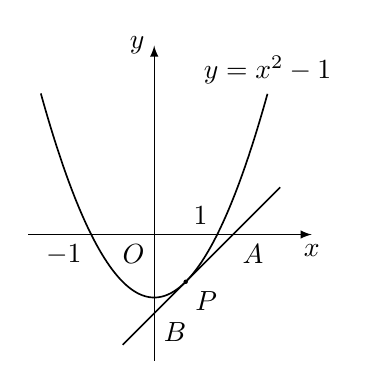
\begin{tikzpicture}[>=latex,scale=0.8]
  \draw[->](-2,0)--(2.5,0)node[below]{$x$};
  \draw[->](0,-2)--(0,3.0)node[left]{$y$};
  \node at (0,0)[below left]{$O$};
  \draw[semithick,samples=200,domain=-1.8:1.8]plot(\x,{\x*\x-1})node[above]{$y=x^2-1$};
  \draw[semithick](-0.5,-1.75)--(2,0.75);
  \node at (1,0)[above left]{$1$};
  \node at (-1,0)[below left]{$-1$};
  \node at (1.25,0)[below right]{$A$};
  \node at (0,-1.25)[below right]{$B$};
  \fill(0.5,-0.75)circle(1pt)node[below right]{$P$};
\end{tikzpicture}
\end{document}